\documentclass[11pt]{article}

\usepackage{amsmath,amssymb,mathtools}
\usepackage[margin=1in]{geometry}
\usepackage{enumitem}
\usepackage{xcolor}
\usepackage{microtype}
\usepackage{graphicx}
\usepackage{tikz,float}
\usepackage{subcaption}
\usepackage{amsthm}
\usepackage{hyperref}
\usepackage{array}
\usepackage{pgfplots}

\usetikzlibrary{shapes.geometric, arrows.meta, positioning, calc, decorations.markings}
\tikzset{
	block/.style={rectangle, draw, text width=6em, text centered, rounded corners, minimum height=10mm},
	sum/.style={circle, draw, node distance=1.5cm},
	line/.style={draw, -{Stealth[length=2.5mm, width=1.5mm]}}
}

\usepgfplotslibrary{groupplots}
\pgfplotsset{compat=1.18}

\pgfplotsset{
	myaxes/.style={
		axis lines=middle,
		axis line style={-latex},
		grid=major,
		grid style={gray!15},
		minor grid style={gray!35},
		xlabel style={at={(ticklabel* cs:1)}, anchor=north west},
		ylabel style={at={(ticklabel* cs:1)}, anchor=south east},
		every axis plot/.append style={thick}
	},
	myplotstyle/.style={
		width=14cm,
		height=7cm,
		axis lines=middle,
		axis line style={-Stealth},
		grid=both,
		minor tick num=1,
		major grid style={draw=gray!30},
		minor grid style={draw=gray!15},
		tick label style={font=\small, fill=white, inner sep=1.5pt},
		xlabel={$t$},
		ylabel={$x(t)$},
		xlabel style={anchor=north east, font=\small},
		ylabel style={anchor=south east, font=\small},
		samples=401,
	}
}

\newtheoremstyle{mynote}
{6pt}      % Space above
{6pt}      % Space below
{}          % Body font (normal, not italic)
{}          % Indent amount
{\bfseries} % Theorem head font
{.}         % Punctuation after theorem head
{.5em}      % Space after theorem head
{}          % Theorem head spec
\theoremstyle{mynote}
\newtheorem{definition}{Definition}
\newtheorem{proposition}{Proposition}
\newtheorem{example}{Example}
\newtheorem{remark}{Remark}
\newtheorem{theorem}{Theorem}
\newtheorem{corollary}{Corollary}

\newcommand{\T}{\mathcal{T}}
\newcommand{\R}{\mathbb{R}}
\newcommand{\Z}{\mathbb{Z}}
\newcommand{\C}{\mathbb{C}}
\newcommand{\conv}{\ast}
\newcommand{\dt}{\,\dd t}
\newcommand{\dd}{\mathrm{d}}
\newcommand{\imp}{\delta}
\newcommand{\sinc}[1]{\frac{\sin(\pi #1)}{\pi #1}}


\DeclareMathOperator{\rect}{rect}
\DeclareMathOperator{\Ev}{Ev}
\DeclareMathOperator{\Od}{Od}
\DeclareMathOperator{\sgn}{sgn}
\DeclareMathOperator{\step}{u}
\DeclareMathOperator{\tri}{tri}


\begin{document}
	% Reset figure counter for this lecture
	\renewcommand{\thefigure}{5.\arabic{figure}}
	
	% --- TITLE BLOCK ---
	\thispagestyle{empty}
	\noindent
	\begin{tabular*}{\textwidth}{l @{\extracolsep{\fill}} r}
		\textbf{Signals and Systems} & \textbf{Lecture 5} \\
		\textit{Dr. Ghandi Manasra and Ahmed Rabei} & \textit{Fall 2025} \\
	\end{tabular*}
	\hrule
	\vspace{0.4cm}
	\begin{center}
		\Large\textbf{Lecture 5: Continuous-Time LTI Systems and the Convolution Integral}
	\end{center}
	\vspace{0.4cm}
	
	\section*{Reference}
	Oppenheim \& Willsky, \textit{Signals and Systems}, Chapter 2, Section 2.2
	
	\section*{Review of Lecture 4}
	\begin{itemize}[noitemsep]
		\item Discrete-time convolution sum derived
		\item Signal decomposition using impulses
		\item LTI systems characterized by impulse response
		\item Flip-and-slide method for computation
	\end{itemize}
	
	Today we extend the convolution concept to continuous-time LTI systems. The derivation and intuition are identical to the discrete-time case—the only difference is that summation becomes integration.
	
	\section*{5.1 Representing CT Signals with Impulses}
	
	Just as in discrete-time, any continuous-time signal can be represented as a linear combination of impulses. Because time is continuous, this "sum" becomes an integral.
	
	\begin{proposition}[Continuous-Time Sifting Property]
		Any continuous-time signal $x(t)$ can be written as:
		\[
		x(t) = \int_{-\infty}^{\infty} x(\tau)\imp(t-\tau) \dd\tau
		\]
	\end{proposition}
	
	
	\paragraph{Intuition:} We can approximate $x(t)$ with narrow rectangular pulses of width $\Delta$ and height $x(k\Delta)$. As $\Delta \to 0$, these pulses become impulses, and the sum becomes an integral. The value $x(\tau)\dd\tau$ is the infinitesimal "weight" of the impulse at time $\tau$.
	\newpage
	\section*{5.2 The Convolution Integral}
	
	Now let's apply this impulse representation to a continuous-time LTI system $\T$. The logic is identical to the discrete-time case.
	
	\begin{align}
	y(t) &= \T\{x(t)\} = \T\left\{\int_{-\infty}^{\infty} x(\tau)\imp(t-\tau) \dd\tau\right\}
	\end{align}
	
	\textbf{Step 1: Use Linearity.} The response to a weighted integral of inputs is the weighted integral of individual responses:
	\[
	y(t) = \int_{-\infty}^{\infty} x(\tau) \T\{\imp(t-\tau)\} \dd\tau
	\]
	
	\textbf{Step 2: Use Time-Invariance.} Define the \textbf{impulse response} $h(t) = \T\{\imp(t)\}$. For an LTI system:
	\[
	\T\{\imp(t-\tau)\} = h(t-\tau)
	\]
	
	\textbf{Step 3: Combine.} Substituting back gives us the \textbf{convolution integral}:
	
	\begin{definition}[Continuous-Time Convolution Integral]
		\[
		y(t) = \int_{-\infty}^{\infty} x(\tau)h(t-\tau) \dd\tau = (x \conv h)(t)
		\]
	\end{definition}
	
	
	\begin{remark}
		The impulse response $h(t)$ completely characterizes any continuous-time LTI system. Given $h(t)$, we can compute the output $y(t)$ for any input $x(t)$. This is \textbf{not} true for nonlinear systems.
	\end{remark}
	
	\section*{5.3 Physical Examples}
	
	\paragraph{1. RC Low-Pass Filter:} 
	The impulse response of an RC circuit is $h(t) = \frac{1}{RC}e^{-t/RC}u(t)$. The output voltage is the convolution of input voltage with this impulse response. The capacitor "remembers" recent inputs more strongly; contributions from the distant past fade exponentially.
	
	\paragraph{2. Mass-Spring-Damper System:} 
	For a mechanical system with mass $m$, spring constant $k$, and damping coefficient $c$, the impulse response is $h(t) = \frac{1}{m\omega_d}e^{-\zeta\omega_n t}\sin(\omega_d t)u(t)$ where $\omega_n = \sqrt{k/m}$, $\zeta = c/(2\sqrt{km})$, and $\omega_d = \omega_n\sqrt{1-\zeta^2}$. The system's response to any force input is the convolution of the force with this impulse response.
	
	\paragraph{3. Heat Diffusion in a Rod:} 
	In a one-dimensional heat conduction problem, if we apply a unit heat pulse at $t=0$ at one end of a rod, the temperature distribution evolves as $h(x,t) = \frac{1}{\sqrt{4\pi\alpha t}}e^{-x^2/(4\alpha t)}u(t)$ where $\alpha$ is thermal diffusivity. The temperature at any point is the convolution of the heat input with this impulse response.
	
	\paragraph{4. Acoustic Echo System:} 
	In a room with hard walls, sound reflects and creates echoes. The impulse response $h(t) = \delta(t) + \alpha\delta(t-T) + \alpha^2\delta(t-2T) + \ldots$ represents the direct sound plus exponentially decaying echoes with delay $T$ and reflection coefficient $\alpha$. The room's response to any sound is the convolution of the input with this impulse response.
	
	\begin{figure}[H]
		\centering
		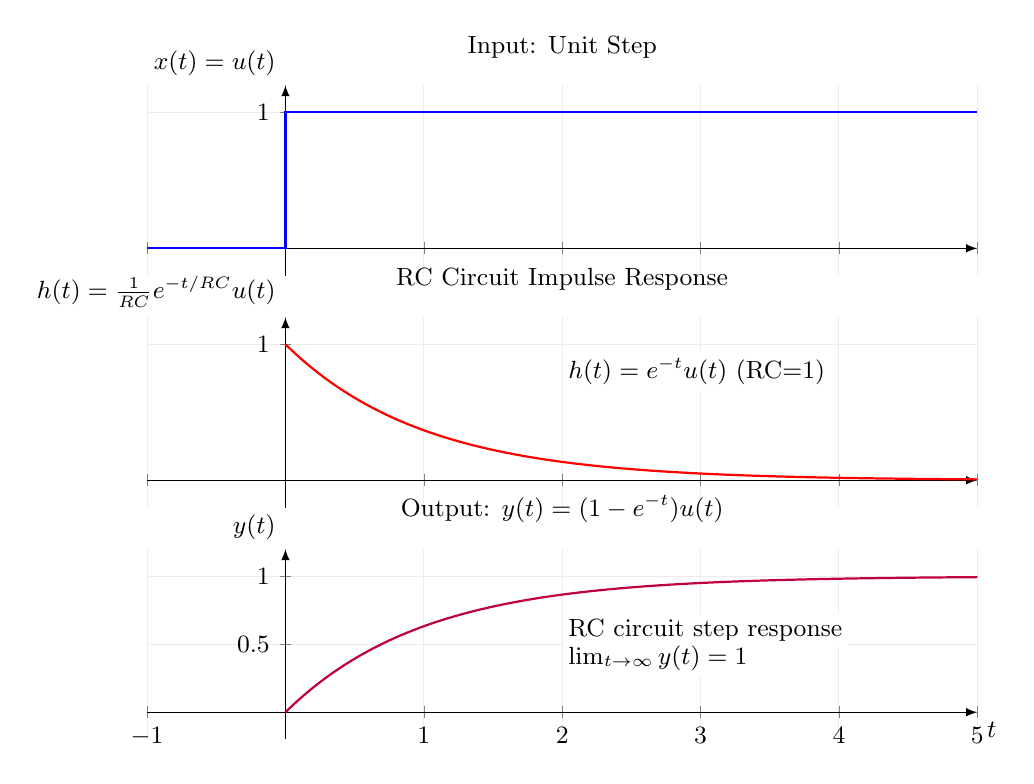
\begin{tikzpicture}
	\begin{groupplot}[
		group style={group size=1 by 3, vertical sep=15pt, xticklabels at=edge bottom},
		/tikz/font=\small,
		width=\linewidth, height=4cm, myaxes,
		xmin=-1, xmax=5,
		domain=-1:5,
		samples=200]
		
		\nextgroupplot[ylabel={$x(t) = u(t)$}, ymin=-0.2, ymax=1.2, ytick={0,1}, title={Input: Unit Step}]
		\addplot[thick, blue] coordinates {
			(-1,0) (0,0) (0,1) (5,1)
		};
		
		\nextgroupplot[ylabel={$h(t) = \frac{1}{RC}e^{-t/RC}u(t)$}, ymin=-0.2, ymax=1.2, ytick={0,1}, title={RC Circuit Impulse Response}]
		\addplot[thick, red, domain=0:5] {exp(-x)};
		\node[anchor=west, fill=white, inner sep=2pt] at (axis cs:2,0.8) 
		{$h(t) = e^{-t}u(t)$ (RC=1)};
		
		\nextgroupplot[xlabel={$t$}, ylabel={$y(t)$}, ymin=-0.2, ymax=1.2, ytick={0,0.5,1}, title={Output: $y(t) = (1-e^{-t})u(t)$}]
		\addplot[thick, purple, domain=0:5] {1 - exp(-x)};
		\node[anchor=west, fill=white, inner sep=2pt] at (axis cs:2,0.6) 
		{RC circuit step response};
		\node[anchor=west, fill=white, inner sep=2pt] at (axis cs:2,0.4) 
		{$\lim_{t \to \infty} y(t) = 1$};
	\end{groupplot}
\end{tikzpicture}

		\caption{RC circuit convolution example with step input.}
		\label{fig:rc_circuit_example}
	\end{figure}
	
	\section*{5.4 Computing Convolution: Flip-and-Slide Method}
	
	To compute convolution at a point $t$:
	
	\begin{enumerate}[noitemsep]
		\item \textbf{Plot signals} $x(\tau)$ and $h(\tau)$ as functions of dummy variable $\tau$.
		\item \textbf{Flip} $h(\tau)$ around zero to get $h(-\tau)$.
		\item \textbf{Slide} $h(-\tau)$ by $t$ to obtain $h(t-\tau)$.
		\item \textbf{Multiply} pointwise: $x(\tau) \times h(t-\tau)$.
		\item \textbf{Integrate} the area under the product curve.
	\end{enumerate}
	
	The integral gives the output $y(t)$ at time $t$.
	\newpage
	\section*{5.5 Numerical Examples}
	
	\begin{example}[Two Rectangular Pulses]
		Given:
		\[
		x(t) = \begin{cases} 1 & 0 \leq t \leq 1 \\ 0 & \text{otherwise} \end{cases}, \qquad 
		h(t) = \begin{cases} 1 & 0 \leq t \leq 1 \\ 0 & \text{otherwise} \end{cases}
		\]
		
		Find $y(t) = (x \conv h)(t)$.
		
		\textbf{Solution:} We need to consider different regions of overlap:
		\begin{itemize}[noitemsep]
			\item $t < 0$: No overlap $\Rightarrow y(t) = 0$
			\item $0 \leq t < 1$: Partial overlap from $\tau = 0$ to $\tau = t$ $\Rightarrow y(t) = t$
			\item $1 \leq t < 2$: Partial overlap from $\tau = t-1$ to $\tau = 1$ $\Rightarrow y(t) = 2-t$
			\item $t \geq 2$: No overlap $\Rightarrow y(t) = 0$
		\end{itemize}
		
		Therefore: $y(t) = \begin{cases} t & 0 \leq t < 1 \\ 2-t & 1 \leq t < 2 \\ 0 & \text{otherwise} \end{cases}$
	\end{example}
	
	\begin{figure}[H]
		\centering
		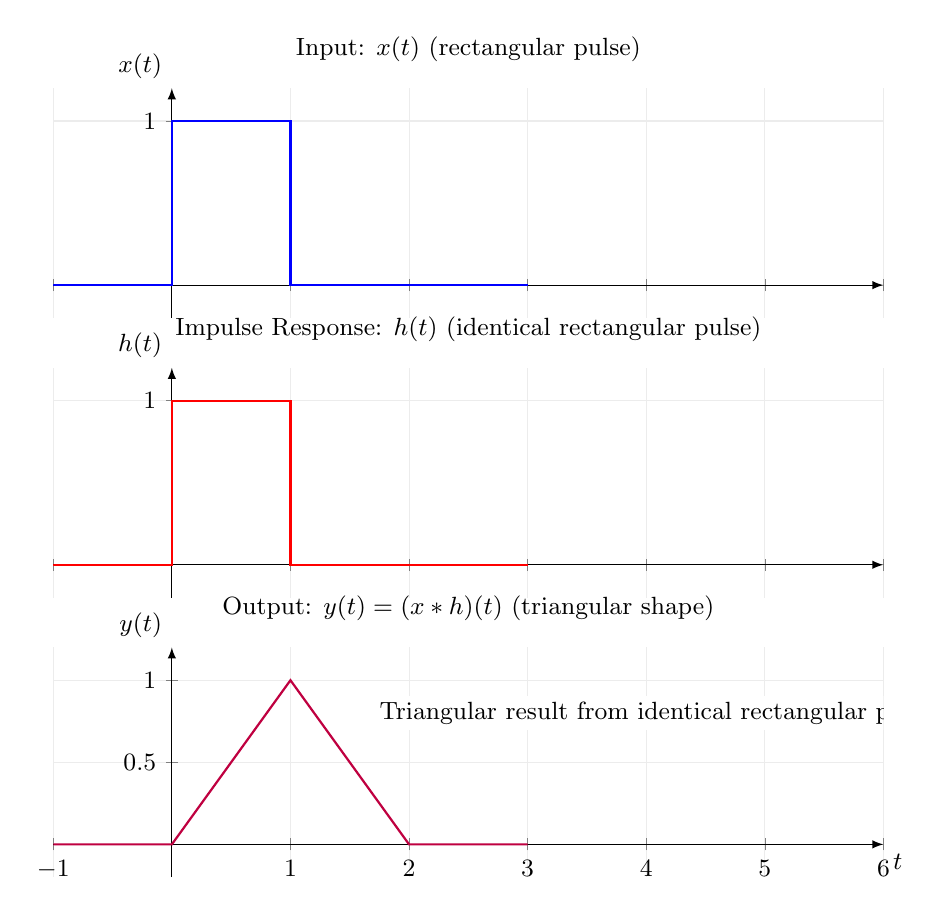
\begin{tikzpicture}
	\begin{groupplot}[
		group style={group size=1 by 3, vertical sep=18pt, xticklabels at=edge bottom},
		/tikz/font=\small,
		width=\linewidth, height=4.5cm, myaxes,
		xmin=-1, xmax=6,
		domain=-1:6,
		samples=200]
		
		\nextgroupplot[ylabel={$x(t)$}, ymin=-0.2, ymax=1.2, ytick={0,1}, title={Input: $x(t)$ (rectangular pulse)}]
		\addplot[thick, blue] coordinates {
			(-1,0) (0,0) (0,1) (1,1) (1,0) (3,0)
		};
		\addplot[thick, blue, const plot] coordinates {
			(-1,0) (0,0) (0,1) (1,1) (1,0) (3,0)
		};
		
		\nextgroupplot[ylabel={$h(t)$}, ymin=-0.2, ymax=1.2, ytick={0,1}, title={Impulse Response: $h(t)$ (identical rectangular pulse)}]
		\addplot[thick, red] coordinates {
			(-1,0) (0,0) (0,1) (1,1) (1,0) (3,0)
		};
		\addplot[thick, red, const plot] coordinates {
			(-1,0) (0,0) (0,1) (1,1) (1,0) (3,0)
		};
		
		\nextgroupplot[xlabel={$t$}, ylabel={$y(t)$}, ymin=-0.2, ymax=1.2, ytick={0,0.5,1}, title={Output: $y(t) = (x \conv h)(t)$ (triangular shape)}]
		\addplot[thick, purple] coordinates {
			(-1,0) (0,0) (1,1) (2,0) (3,0)
		};
		\node[anchor=west, fill=white, inner sep=2pt] at (axis cs:1.7,0.8) 
		{Triangular result from identical rectangular pulses};
	\end{groupplot}
\end{tikzpicture}

		\caption{Convolution of two identical rectangular pulses showing triangular result.}
		\label{fig:rectangular_convolution}
	\end{figure}
	\newpage
	\begin{example}[Exponential with Delayed Step]
		Given:
		\[
		x(t) = e^{-t}u(t), \qquad h(t) = u(t-1)
		\]
		
		Find $y(t) = (x \conv h)(t)$.
		
		\textbf{Solution:}
		\begin{align}
		y(t) &= \int_{-\infty}^{\infty} e^{-\tau}u(\tau) \cdot u(t-\tau-1) \dd\tau
		\end{align}
		
		Since $u(\tau) = 0$ for $\tau < 0$ and $u(t-\tau-1) = 0$ for $\tau > t-1$:
		\begin{itemize}[noitemsep]
			\item If $t < 1$: No overlap $\Rightarrow y(t) = 0$
			\item If $t \geq 1$: Integrate from $\tau = 0$ to $\tau = t-1$
		\end{itemize}
		
		For $t \geq 1$:
		\begin{align}
		y(t) &= \int_{0}^{t-1} e^{-\tau} \dd\tau = \left[-e^{-\tau}\right]_0^{t-1} = 1 - e^{-(t-1)}
		\end{align}
		
		Therefore: $y(t) = (1-e^{-(t-1)})u(t-1)$
	\end{example}
	
	\begin{figure}[H]
		\centering
		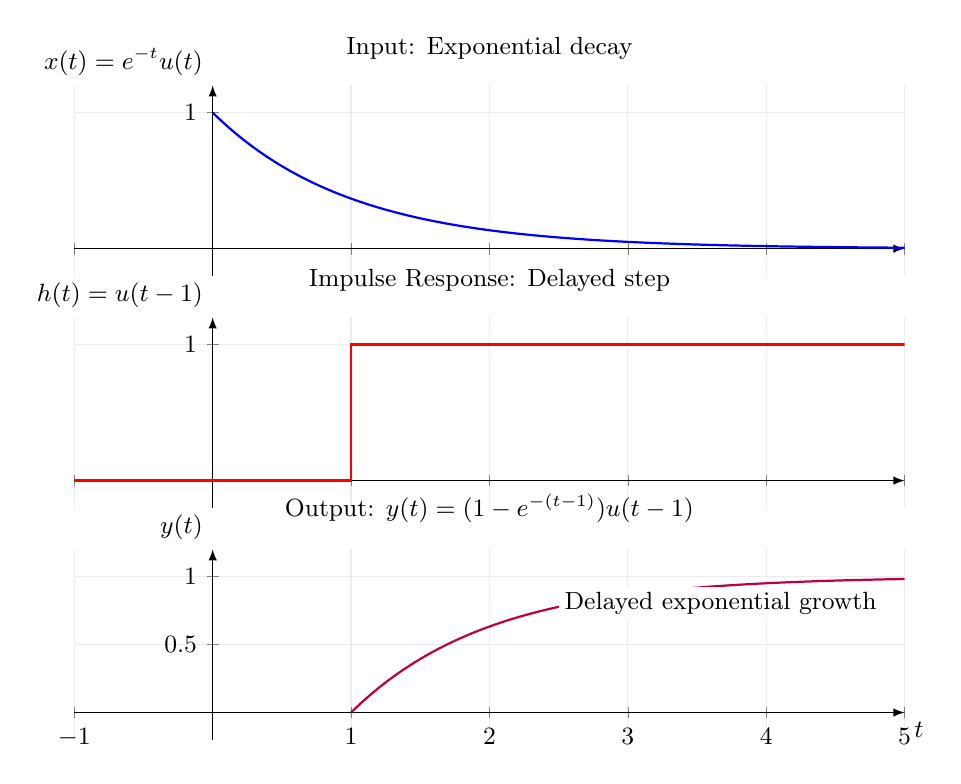
\begin{tikzpicture}
	\begin{groupplot}[
		group style={group size=1 by 3, vertical sep=15pt, xticklabels at=edge bottom},
		/tikz/font=\small,
		width=\linewidth, height=4cm, myaxes,
		xmin=-1, xmax=5,
		domain=-1:5,
		samples=200]
		
		\nextgroupplot[ylabel={$x(t) = e^{-t}u(t)$}, ymin=-0.2, ymax=1.2, ytick={0,1}, title={Input: Exponential decay}]
		\addplot[thick, blue, domain=0:5] {exp(-x)};
		
		\nextgroupplot[ylabel={$h(t) = u(t-1)$}, ymin=-0.2, ymax=1.2, ytick={0,1}, title={Impulse Response: Delayed step}]
		\addplot[thick, red] coordinates {
			(-1,0) (1,0) (1,1) (5,1)
		};
		
		\nextgroupplot[xlabel={$t$}, ylabel={$y(t)$}, ymin=-0.2, ymax=1.2, ytick={0,0.5,1}, title={Output: $y(t) = (1-e^{-(t-1)})u(t-1)$}]
		\addplot[thick, purple, domain=1:5] {1 - exp(-(x-1))};
		\node[anchor=west, fill=white, inner sep=2pt] at (axis cs:2.5,0.8) 
		{Delayed exponential growth};
	\end{groupplot}
\end{tikzpicture}

		\caption{Convolution of exponential with delayed step function.}
		\label{fig:exponential_delayed_step}
	\end{figure}
	\newpage
	\begin{example}[Two Exponentials with Different Decay Rates]
		Given:
		\[
		x(t) = e^{-2t}u(t), \qquad h(t) = e^{-3t}u(t)
		\]
		
		Find $y(t) = (x \conv h)(t)$.
		
		\textbf{Solution:}
		\begin{align}
		y(t) &= \int_{-\infty}^{\infty} e^{-2\tau}u(\tau) \cdot e^{-3(t-\tau)}u(t-\tau) \dd\tau
		\end{align}
		
		For $t \geq 0$:
		\begin{align}
		y(t) &= \int_{0}^{t} e^{-2\tau} \cdot e^{-3(t-\tau)} \dd\tau = e^{-3t} \int_{0}^{t} e^{\tau} \dd\tau \\
		&= e^{-3t} \left[e^{\tau}\right]_0^t = e^{-3t}(e^t - 1) = e^{-2t} - e^{-3t}
		\end{align}
		
		Therefore: $y(t) = (e^{-2t} - e^{-3t})u(t)$
	\end{example}
	
	\begin{figure}[H]
		\centering
		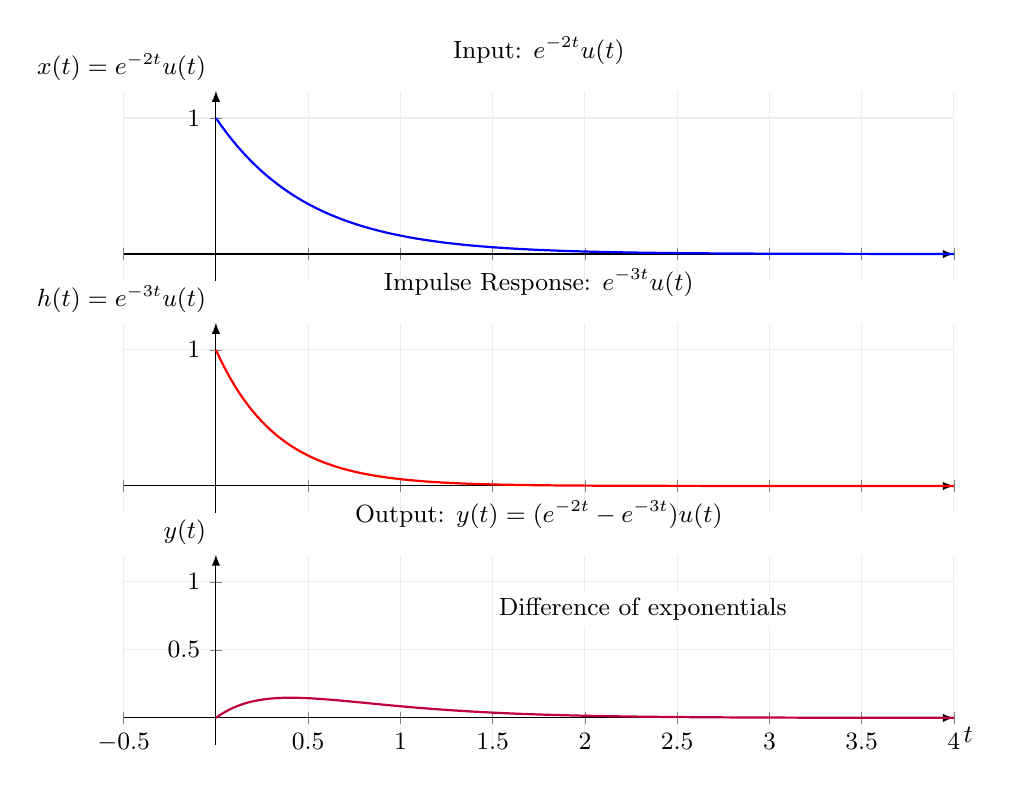
\begin{tikzpicture}
	\begin{groupplot}[
		group style={group size=1 by 3, vertical sep=15pt, xticklabels at=edge bottom},
		/tikz/font=\small,
		width=\linewidth, height=4cm, myaxes,
		xmin=-0.5, xmax=4,
		domain=-0.5:4,
		samples=200]
		
		\nextgroupplot[ylabel={$x(t) = e^{-2t}u(t)$}, ymin=-0.2, ymax=1.2, ytick={0,1}, title={Input: $e^{-2t}u(t)$}]
		\addplot[thick, blue, domain=0:4] {exp(-2*x)};
		
		\nextgroupplot[ylabel={$h(t) = e^{-3t}u(t)$}, ymin=-0.2, ymax=1.2, ytick={0,1}, title={Impulse Response: $e^{-3t}u(t)$}]
		\addplot[thick, red, domain=0:4] {exp(-3*x)};
		
		\nextgroupplot[xlabel={$t$}, ylabel={$y(t)$}, ymin=-0.2, ymax=1.2, ytick={0,0.5,1}, title={Output: $y(t) = (e^{-2t} - e^{-3t})u(t)$}]
		\addplot[thick, purple, domain=0:4] {exp(-2*x) - exp(-3*x)};
		\node[anchor=west, fill=white, inner sep=2pt] at (axis cs:1.5,0.8) 
		{Difference of exponentials};
	\end{groupplot}
\end{tikzpicture}

		\caption{Convolution of two exponential functions with different decay rates.}
		\label{fig:two_exponentials}
	\end{figure}
	\newpage
	\begin{example}[Impulse Train with Exponential]
		Given:
		\[
		x(t) = \sum_{n=0}^{2} \imp(t-n), \qquad h(t) = e^{-t}u(t)
		\]
		
		Find $y(t) = (x \conv h)(t)$.
		
		\textbf{Solution:} Using the fact that convolution with impulses gives shifted impulse responses:
		\begin{align}
		y(t) &= \sum_{n=0}^{2} h(t-n) = \sum_{n=0}^{2} e^{-(t-n)}u(t-n)
		\end{align}
		
		This gives:
		\begin{itemize}[noitemsep]
			\item $t < 0$: $y(t) = 0$
			\item $0 \leq t < 1$: $y(t) = e^{-t}$
			\item $1 \leq t < 2$: $y(t) = e^{-t} + e^{-(t-1)} = e^{-t}(1 + e)$
			\item $t \geq 2$: $y(t) = e^{-t} + e^{-(t-1)} + e^{-(t-2)} = e^{-t}(1 + e + e^2)$
		\end{itemize}
	\end{example}
	
	\begin{figure}[H]
		\centering
		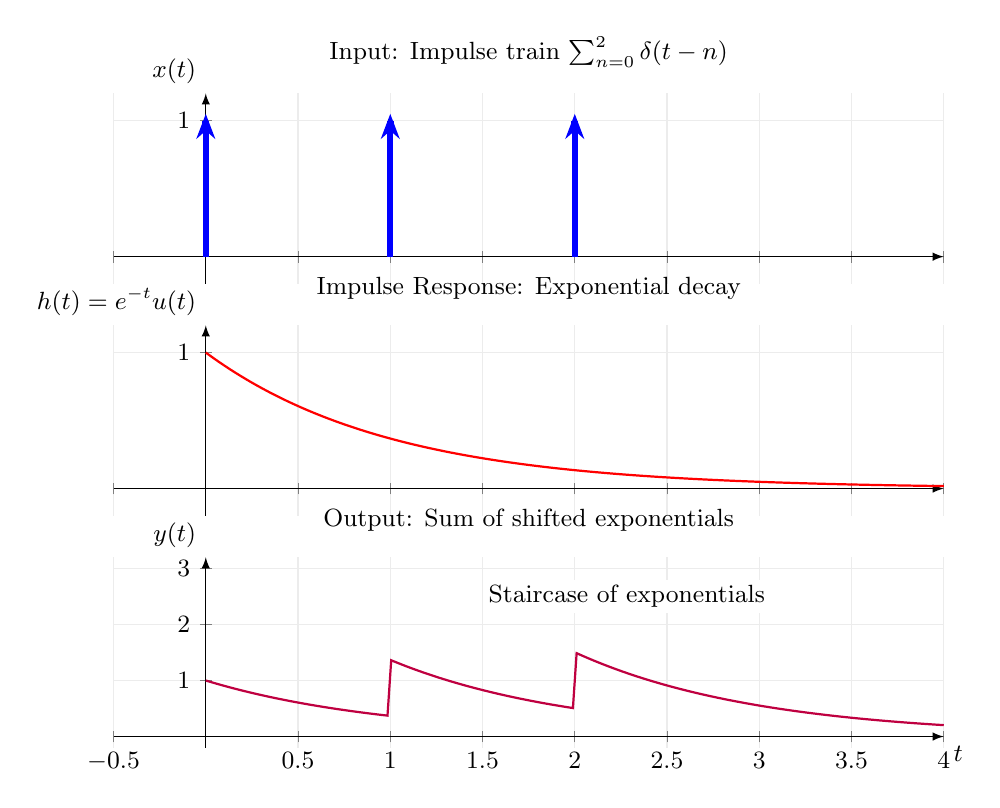
\begin{tikzpicture}
	\begin{groupplot}[
		group style={group size=1 by 3, vertical sep=15pt, xticklabels at=edge bottom},
		/tikz/font=\small,
		width=\linewidth, height=4cm, myaxes,
		xmin=-0.5, xmax=4,
		domain=-0.5:4,
		samples=200]
		
		\nextgroupplot[ylabel={$x(t)$}, ymin=-0.2, ymax=1.2, ytick={0,1}, title={Input: Impulse train $\sum_{n=0}^{2}\delta(t-n)$}]
		\draw[blue, line width=2.2pt] (axis cs:0,0) -- (axis cs:0,1);
		\draw[blue, line width=2.6pt, -{Stealth[length=9pt]}] (axis cs:0,1) -- (axis cs:0,1.05);
		\draw[blue, line width=2.2pt] (axis cs:1,0) -- (axis cs:1,1);
		\draw[blue, line width=2.6pt, -{Stealth[length=9pt]}] (axis cs:1,1) -- (axis cs:1,1.05);
		\draw[blue, line width=2.2pt] (axis cs:2,0) -- (axis cs:2,1);
		\draw[blue, line width=2.6pt, -{Stealth[length=9pt]}] (axis cs:2,1) -- (axis cs:2,1.05);
		
		\nextgroupplot[ylabel={$h(t) = e^{-t}u(t)$}, ymin=-0.2, ymax=1.2, ytick={0,1}, title={Impulse Response: Exponential decay}]
		\addplot[thick, red, domain=0:4] {exp(-x)};
		
		\nextgroupplot[xlabel={$t$}, ylabel={$y(t)$}, ymin=-0.2, ymax=3.2, ytick={0,1,2,3}, title={Output: Sum of shifted exponentials}]
		\addplot[thick, purple, domain=0:4] {exp(-x) + (x >= 1) * exp(-(x-1)) + (x >= 2) * exp(-(x-2))};
		\node[anchor=west, fill=white, inner sep=2pt] at (axis cs:1.5,2.5) 
		{Staircase of exponentials};
	\end{groupplot}
\end{tikzpicture}

		\caption{Convolution of impulse train with exponential function.}
		\label{fig:impulse_train_exponential}
	\end{figure}
	
	\section*{Summary and Next Lecture}
	\begin{itemize}[noitemsep]
		\item Continuous-time signals decompose into impulse integrals.
		\item CT LTI system output is convolution integral: $y(t) = \int x(\tau)h(t-\tau) \dd\tau$.
		\item Impulse response $h(t)$ completely characterizes CT LTI systems.
		\item Convolution computed using flip-and-slide method with integration.
		\item \textbf{Next time:} Properties of convolution and LTI system characteristics.
	\end{itemize}
	
\end{document}
